\newcommand{\h}{handout,%
}

\documentclass[
\h%
ucs,ignorenonframetext,hyperref={pdftex,unicode},xcolor=dvipsnames]{beamer}
\usepackage[utf8x]{inputenc}
\usepackage[russian]{babel}
\usepackage[T2A]{fontenc}
\usepackage{tikz}
\usetikzlibrary{shapes,arrows,positioning,chains,calc}
\usepackage{graphicx}
\usepackage{fixltx2e}
\usepackage{paratype}
\usepackage{booktabs}
\usepackage{xcolor}
\usepackage{pbox}

\newcommand{\screenshot}[1]{
\begin{center}
\includegraphics[width=12cm,keepaspectratio]{./images/#1}
\end{center}
}

\newcommand{\screenshotw}[2]{
\begin{center}
\includegraphics[width=#1,keepaspectratio]{./images/#2}
\end{center}
}

\usecolortheme{crane}
\useoutertheme{infolines}
\setbeamertemplate{navigation symbols}{}

\author[А. М. Пеленицын]{А.~М.~Пеленицын\texorpdfstring{\\}{ }
apel@sfedu.ru}

\date{Весна 2016}

\institute[Мехмат ЮФУ]{Южный федеральный университет \texorpdfstring{\\}{ }
Институт математики, механики и компьютерных наук им. И.\,И.~Воровича\texorpdfstring{\\}{ }
Кафедра информатики и вычислительного эксперимента}

\subtitle{}

\AtBeginSection[]
{
\begin{frame}<beamer>
\frametitle{Содержание}
\tableofcontents[currentsection,hideothersubsections]
\end{frame}
}

\AtBeginSubsection[]
{
\begin{frame}<beamer>
\frametitle{Содержание}
\tableofcontents[currentsection,subsectionstyle=show/shaded/hide]
\end{frame}
}

\newcommand{\nspace}{\hspace{0pt}}
\newcommand{\nbdash}{\nobreakdash-\nspace}
\newcommand{\up}{\textsuperscript}
\newcommand{\bslash}{\textbackslash}

\newcommand{\link}[2]{\textcolor{blue}{\href{#1}{#2}}}

\newcommand{\Wrapped}[2][c]{%
  \begin{tabular}[#1]{@{}c@{}}#2\end{tabular}}


\title[Архитектура компьютеров. Лекция 2]{Архитектура компьютеров\texorpdfstring{\\}{ }Лекция 2. Развитие вычислительной техники}

\begin{document}

\begin{frame}
\titlepage
\end{frame}

\section {Развитие вычислительной техники}

\begin{frame}{Поколения компьютерной техники}
\begin{itemize}
    \item Нулевое поколение — (электро-)механические компьютеры (1642–1945)
    \item Первое поколение — электронные лампы (1945–1955)
    \item Второе поколение — транзисторы (1955–1965)
    \item Третье поколение — интегральные схемы (1965–1980)
    \item Четвёртое поколение — СБИС, микропроцессоры, персональные компьютеры (1980+s)
\end{itemize}
\end{frame}

\subsection {(0) Механические компьютеры}

\begin{frame}{Машина Паскаля «Паскалина» (1642)}
    \begin{columns}
    \column{4cm}
        \begin{block}{Блез Паскаль (1623–1662)}
        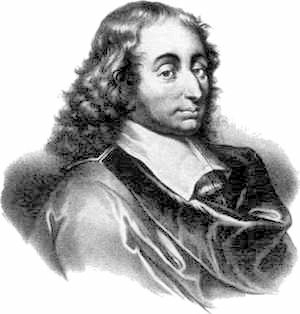
\includegraphics[width=4cm,keepaspectratio]{./images/pascal.jpg}
        \end{block}
    \column{7cm} 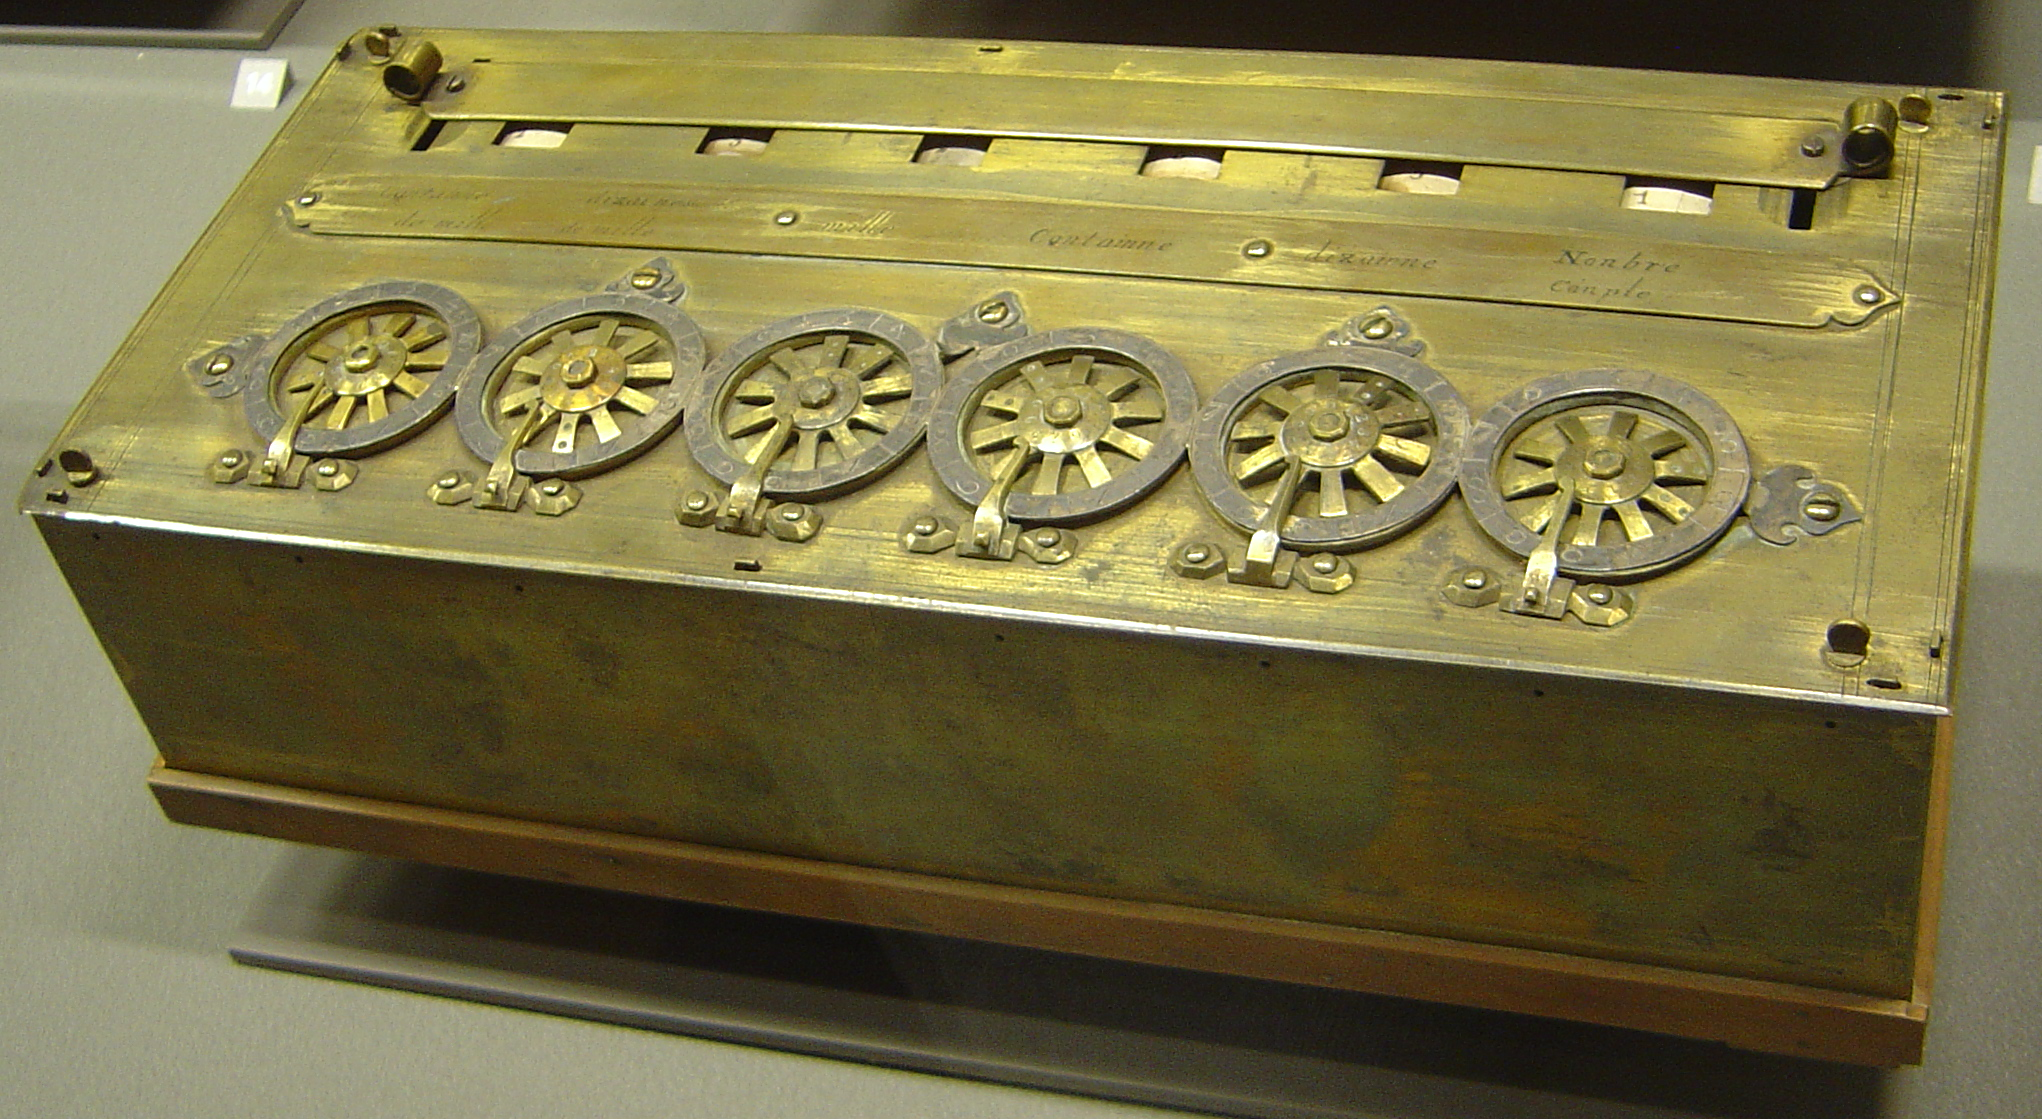
\includegraphics[width=7cm,keepaspectratio]{./images/pascaline.jpg}

    Десятичная система,\\сложение и вычитание
    \end{columns}
\end{frame}

\begin{frame}{Арифмометр Лейбница (вторая половина XVII в.)}
    \begin{columns}
    \column{3.7cm}
        \begin{block}{\small Готфрид Вильгельм Лейбниц (1646–1716)}
            \centering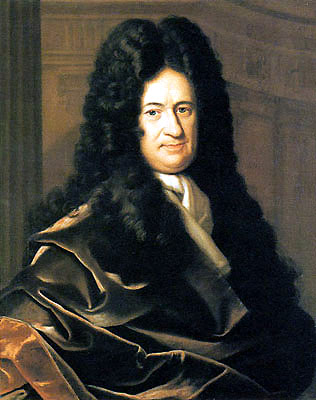
\includegraphics[width=3.5cm,keepaspectratio]{./images/leibniz.jpg}
            %\screenshotw{3.5cm}{leibniz.jpg}
        \end{block}

    \column{7.5cm}

\begin{block}{Stepped Reckoner}
%        \screenshotw{6cm}{leibnitzrechenmaschine.jpg}
            \centering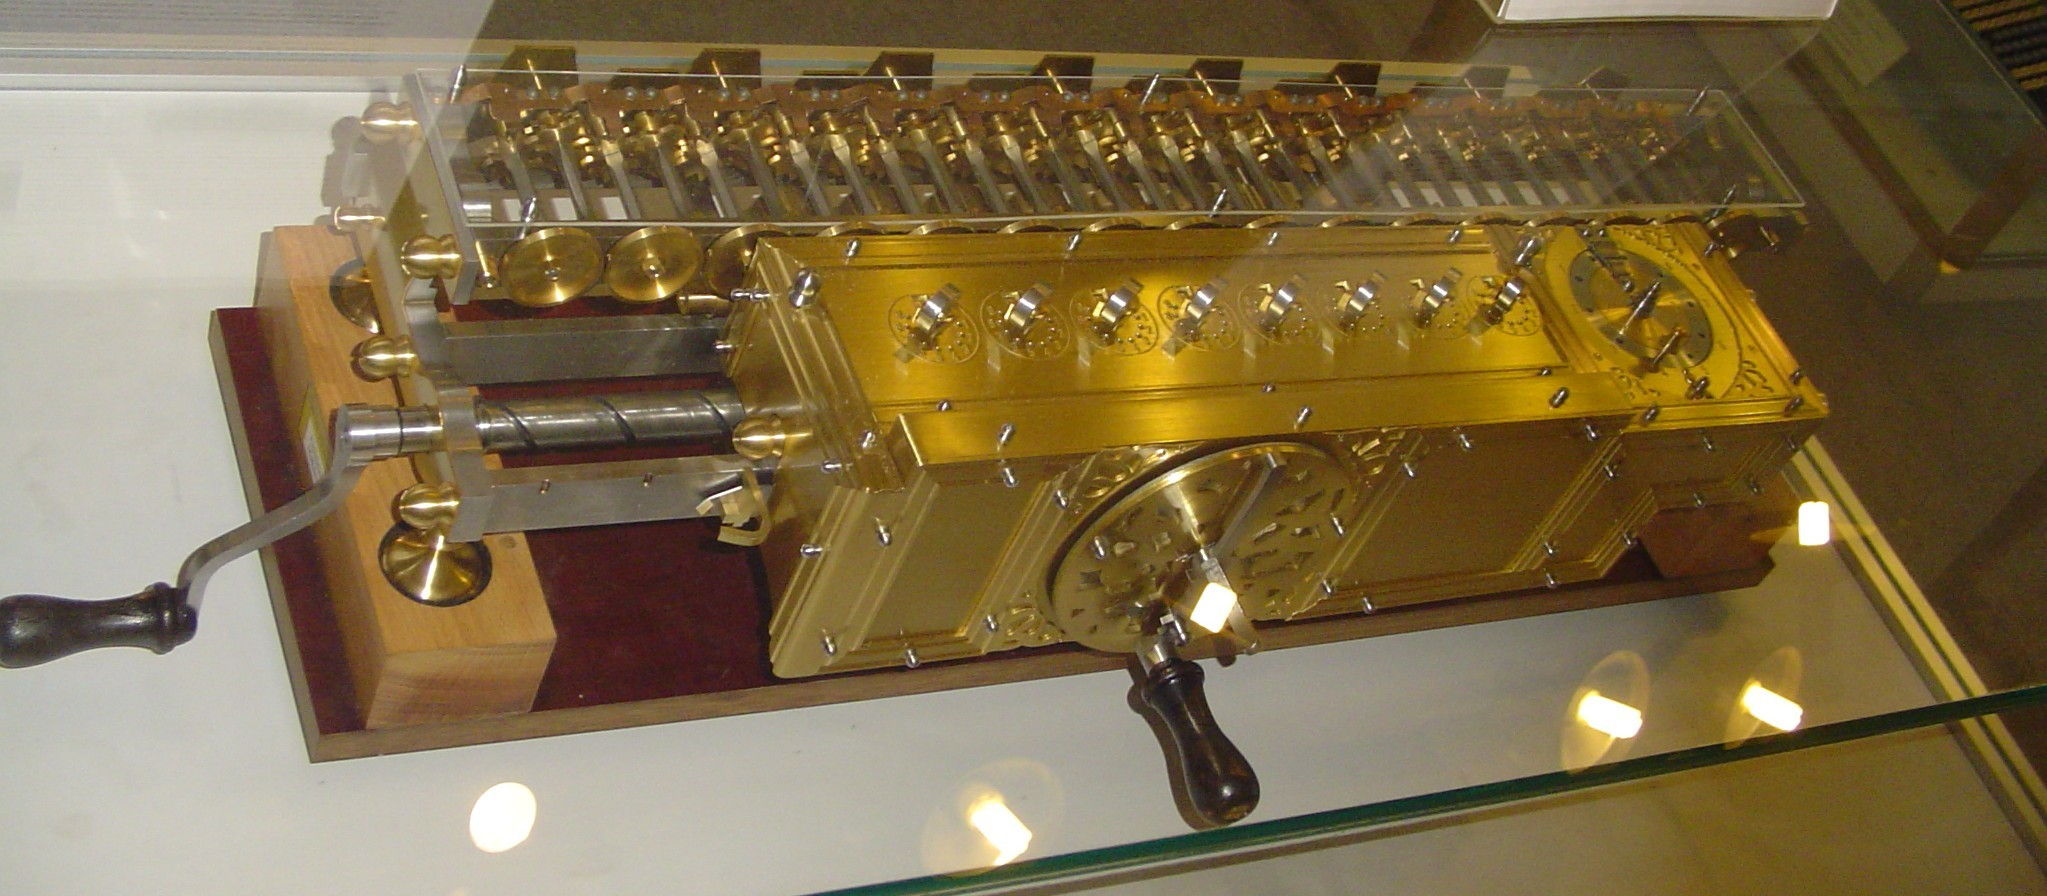
\includegraphics[width=6cm,keepaspectratio]{./images/leibnitzrechenmaschine.jpg}

    \small \par Десятичная система;\\
        сложение, вычитание, умножение, деление.
\end{block}

%    \vspace{.7cm}

    \small
    \onslide<2->{%
    \alert{Двоичная} система.}
    \end{columns}
\begin{quote}
    \small “[...] it is beneath the dignity of excellent men to waste their time in calculation when any peasant could do the work just as accurately with the aid of a machine.”
\end{quote}
\end{frame}

\begin{frame}{Разностная машина (1822)}
    \begin{columns}
    \column{4cm}
        \begin{block}{Чарльз Бэббидж (1791–1871)}
        \screenshotw{4cm}{babbage.jpg}
        \end{block}

    \column{7cm}
        \screenshotw{6.8cm}{DifferenceEngine.jpg}

        Десятичная система,\\
        сложение и вычитание,\\
        результаты выдавливались\\на медной дощечке.
    \end{columns}
\end{frame}

\begin{frame}{Аналитическая машина}
    \begin{columns}
    \column{4.8cm}
        \onslide<2->{
        \begin{block}{Первый программист:\\Ада Лавлейс (1815–1852)}
        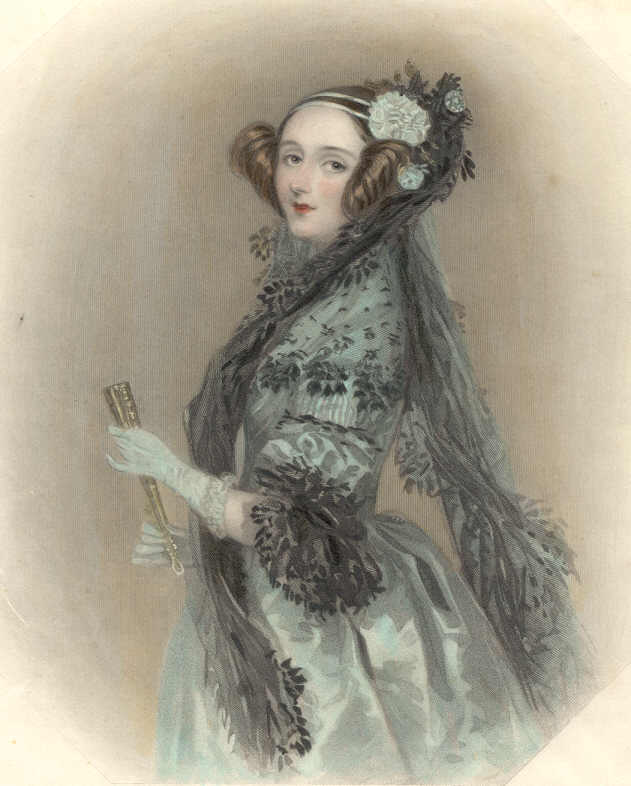
\includegraphics[width=4.7cm,keepaspectratio]{./images/ada.jpg}
        \end{block}}

    \column{6.5cm}
    \begin{itemize}
    \item Автор проекта: Ч. Бэббидж.
    \item Программируемая машина:
        \begin{itemize}
            \item память, \item АЛУ,\item УУ (условия, циклы),
            \item I/O (перфокарты).
        \end{itemize}
        \onslide<3>{\item Luigi Menabrea, 1843,\\
        “Sketch of the Analytical Engine”.}
    \end{itemize}
    \end{columns}
\end{frame}

\begin{frame}{XX в. до 1945 г.}
\pause
\begin{block}{Электро-механические и первые электронные машины}
\begin{itemize}\itemsep=1cm
    \item Z3 (1941) — Конрад Цузе, Германия;
        \\ \onslide<3->{{\small двоичная, плавающая точка, булева логика,
             без ветвлений.}}
    \item Компьютер Атанасова-Берри (ABC, 1942), США;
        \\ \onslide<4->{{\small двоичная, электронная, конденсаторы для памяти, решает СЛУ.}}

    \item Harvard Mark I (1944) — Говард Айкен, IBM;
        \\ \onslide<5->{{\small десятичная, см.~Ч.~Бэббидж, «гарвардская архитектура», “loops”.}}

\end{itemize}
\end{block}
\end{frame}

\subsection {(1) Электронные ламповые компьютеры}

\begin{frame}{Электронные ламповые компьютеры}
\begin{itemize}[<+->]
    \item Colossus (1943/4) — Англия, секретная разработка; dec.
    \item ENIAC (1946)~— США, Д.~Мокли, Д.~П.~Эккерт; \\
    {\small dec; 18000 ламп, 1500 реле, вес 30 тонн; “When Computers Were Women”.}
    \item «Фоннеймановская архитектура»: {\small EDVAC, IAS, EDSAC, UNIVAC…}
    \item Manchester SSEM (“Baby”, 1948) — 1\textsuperscript{st} stored-program.
    \item МЭСМ (1950) — СССР, Киев, лаборатория С.А.~Лебедева.
    \item IBM: 701 (1953), 704 (1956, аппаратная плавающая точка), 709.
\end{itemize}
\end{frame}

\begin{frame}{«Архитектура фон Неймана»}
“First Draft of a Report on the EDVAC”\\
{\small (1945, автор: Д. Фон Нейман, распространитель: Г. Голдстайн)}
\screenshotw{6cm}{fonneiman.png}
%\vspace{-.3cm}
\pause Машина IAS:
\begin{itemize}
    \item память = 4096 слов по 40 бит,
    \item слово = (две команды по 20 бит | целое со знаком на 40 бит),
    \item команда = (8 бит: тип команды) + (12 бит: адрес в памяти).
\end{itemize}
\end{frame}

\subsection {(2) Транзисторные компьютеры}

\begin{frame}{Транзисторы (1947 г.): Нобелевская премия 1956 г.}
\screenshotw{8.5cm}{Bardeen_Shockley_Brattain_1948.JPG}
\vspace{-.3cm}\small Джон Бардин, Уильям Шокли и Уолтер Браттейн в лаборатории Bell, 1948 г.
\end{frame}

\begin{frame}{Транзисторные компьютеры}
\pause
\begin{itemize}[<+->]
    \item PDP-1 (1961) — DEC;\\
        {\small миникомпьютер, \$120'000, дисплей, “Spacewar” (MIT).}

    \item 7090 (1959), 7094~— IBM;\\
        {\small двоичная арифметика, слово = $48$ бит.}

    \item 1401 (1959)~— IBM;\\
        {\small финансовые расчёты, десятичная арифметика,\\
        нет регистров и, как следствие, фиксированной длины слова.}

    \item 6600 (1964)~— CDC;\\
        {\small Сеймур Крей и его «суперкомпьютеры».}
\end{itemize}

\pause
\begin{block}{Мейнфреймы: «IBM и 7 гномов»}
Burroughs, UNIVAC, NCR, Control Data, Honeywell, General Electric, RCA.
\end{block}
\end{frame}

\begin{frame}{Общая шина (omnibus) PDP-8, 1965}
\screenshotw{12cm}{omnibus.png}
12-разрядный, \$16'000, продано около 50'000 экземпляров
\end{frame}

\subsection {(3) Компьютеры на интегральных схемах}

\begin{frame}{Интегральные схемы}
\screenshotw{4.5cm}{chips.jpg}
\vspace{-.3cm}
Изобретатели: Джон Килби, Роберт Нойс и др. (\link{https://en.wikipedia.org/wiki/Invention_of_the_integrated_circuit}{В.: история})\\
Одна микросхема = десятки транзисторов.
\end{frame}

\begin{frame}{IBM System/360 (1965)}
\begin{columns}
    \column{6cm}
\begin{itemize}[<+->]
    \item Идея линейки компьютеров:\\модель 30, 40, 65, 75…,
    \item единый ассемблер,
    \item эмуляция 1401 и 7094 (микропрограммирование),
    \item 16 регистров по 32 разряда и\\
        память, разбитая на \alert{байты},
    \item адресное пространство:\\
        \onslide<6->{$2^{24}$ = 16 Мб — промах!}
\end{itemize}

%\onslide<7->{
%\begin{block}{Пример: инструкция MVC\\(Move Characters), код D2}
%D2FF 8001 7000
%\end{block}}

    \column{5cm}
\screenshotw{5cm}{IBM_System_360-50_console.jpg}
\end{columns}


\end{frame}

\begin{frame}{DEC PDP-11 (1970)}
\begin{columns}
    \column{7cm}
\begin{itemize}%[<+->]
    \item «Младший брат» 360,
    \item линейка машин,
    \item 16-разрядная архитектура,
    \item ортогональный набор инструкций,
    \item memory-mapped I/O, unibus,
    \item \link{http://youtu.be/dFUlAQZB9Ng}{“It's a UNIX system — I know this”}.
\end{itemize}

    \column{5cm}
\screenshotw{4cm}{PDP-11.jpg}
\end{columns}
\end{frame}

\subsection {(4) Современные компьютеры}

\begin{frame}{(4) Персональные компьютеры (микрокомпьютеры)}
\begin{block}{Джон Мокли, New York Times, 1962}
    \textit{There is no reason to suppose the average boy or girl cannot be master of a personal computer.}
\end{block}
\pause
\begin{itemize}
    \item СБИС (\textbf{VLSI}): одна микросхема = десятки тысяч транзисторов,
    \item Intel 8080 (1974): Altair,
    \item Троица (1977 г.): PET, Apple II, TRS-80,
    \item IBM PC @ Intel 8088 (1981 г.): MS-DOS, OS/2, Windows…
    \item IBM-compatibles,
    \item Intel x86.
\end{itemize}
\end{frame}

\end{document}
